
\documentclass[a4paper,12pt,notitlepage]{article}

\usepackage[utf8x]{inputenc}
\usepackage[T1]{fontenc}
\usepackage[francais]{babel}
\usepackage{amssymb,amsmath}
\usepackage{fullpage}
\usepackage[final]{pdfpages}
\usepackage{float}

\title{Calculer une Force}
\date{24.09.2013}
\author{
    Florian Reinhard\\
    florian.reinhard@epfl.ch
}

\begin{document}
    \maketitle

    \section{Marche à suivre}
    \begin{enumerate}
        \item Est-ce que je peux appliquer Laplace?
        \item Est-ce qu'on connaît la distribution du champ magnétique dans
            l'entre fer? -> forme simplifiée du tenseur de Maxwell
        \item Le système est-il linéaire?
            \begin{equation}
                F_m = \frac{1}{2}\sum^k_{j=1} \sum^k_{p=1}\frac{dL_{jp}}{dx_m}i_j i_p
            \end{equation}
        \item Le système est saturable et ne peut pas être résolu par Maxwell
            -> calcul de la dérivée de l'énergie dans l'entrefer si possible ou
            calcul de la dérivée de la coénergie du système complet.
    \end{enumerate}


    \section{Exemple}
    \begin{figure}[H]
        \centering
        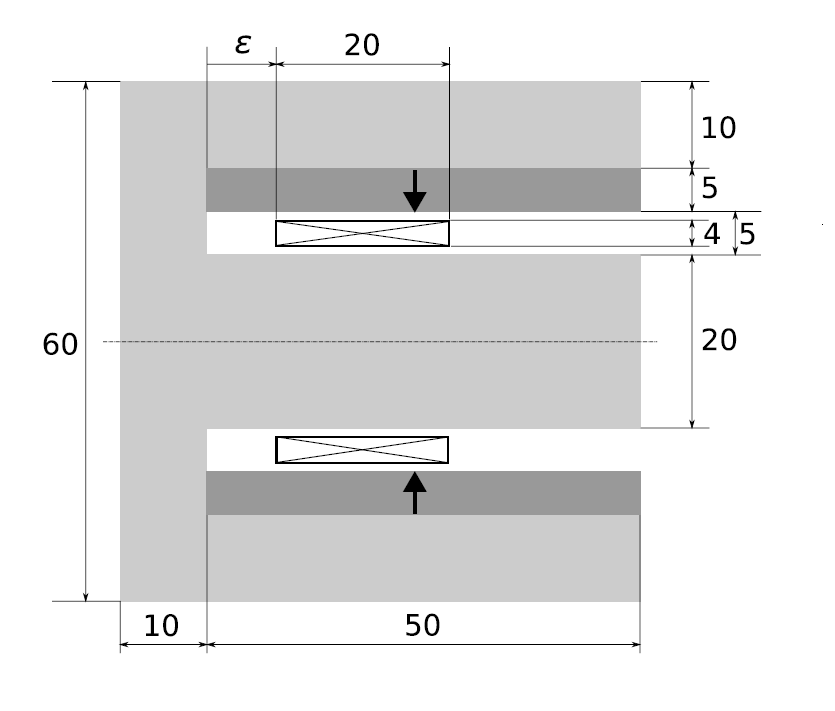
\includegraphics[width=12cm]{exemple_systeme_electrodynamique.png}
        \caption{Exemple d'un système électrodynamique.}
    \end{figure}

    \paragraph{Hypothèses:}
    \begin{itemize}
        \item pas de fuite/franges
        \item pas de saturation et du fer idéal ($ \mu_{fe}=\infty $)
        \item pas d'effets d'extrémités
    \end{itemize}


    \subsection{Laplace}
    \paragraph{Laplace}
    \begin{equation}
        d \vec{F} = I d \vec{l} \times \vec{B}
    \end{equation}

    \paragraph{Champ dans l'entrefer}
    \begin{equation}
        B_{\delta} = B_a = B_0 \frac{\Lambda_e}{\Lambda_e + \Lambda_a}
    \end{equation}

    \begin{equation}
        \Lambda_e = \Lambda_{\delta} = \frac{\mu_0 A_{\delta}}{\delta}
    \end{equation}

    \begin{equation}
        \Lambda_a = \frac{\mu_0 \mu_{dr} A_a}{l_a}
    \end{equation}

    \begin{table}[H]
        \begin{tabular}{c c l}
            $ \Lambda_e $ & : & permanence de l'entrefer \\
            $ \Lambda_a $ & : & permanence interne de l'aimant \\
            $ A_a $ & : & surface de l'aimant \\
            $ A_{\delta} $ & : & surface de l'entrefer \\
            $ l_a $ & : & longueur de l'aimant \\
            $ \delta $ & : & longueur de l'entrefer \\
        \end{tabular}
    \end{table}

    Les permanences $ \Lambda_e $ et $ \Lambda_a $ fonctionnent comme un diviseur
    de tension (mais avec un champ magnétique) sur $ B_0 $.

    \begin{equation}
        B_{\delta} = B_0 \frac{\mu_0 \frac{A_{\delta}}{\delta}}
                {\frac{\mu_0 A_{\delta}}{\delta} + \mu_0 \mu_{dr} \frac{A_a}{l_a}}    
                = B_0 \frac{l_a}{l_a + \mu_{dr} \delta}
    \end{equation}

    \paragraph{Finalement}
    \begin{equation}
        F = I \int B_{\delta} d \vec{l} = I 2 N B_{\delta} h
    \end{equation}

    \begin{table}[H]
        \begin{tabular}{c c l}
            $ h $ & : & profondeur du système \\
        \end{tabular}
    \end{table}


    \subsection{Maxwell}
    \begin{equation}
        F_{\perp} = \mu H_n H_t
    \end{equation}

    Ne marche pas. I.e. trop difficile à calculer.


    \subsection{Dérivée de l'énergie (mal adapté à la électrodynamique)}
    Linéaire, alors:

    \begin{equation}
        F_x = \frac{1}{2} \frac{d\Lambda_{aa}}{dx}\Theta_a^2
        + \frac{d\Lambda_{ab}}{dx}\Theta_a \Theta_b
        + \frac{1}{2} \frac{d\Lambda_{bb}}{dx}\Theta_b^2
    \end{equation}

    \subsubsection{$ \frac{d\Lambda_{aa}}{dx} = ?$ (partie aimant)}
    \begin{equation}
        \Lambda_{aa} = \Lambda_{interne} + \Lambda_{\delta} = const.
    \end{equation}

    \begin{equation}
        \frac{d\Lambda_{aa}}{dx} = 0    
    \end{equation}


    \subsubsection{$ \frac{d\Lambda_{bb}}{dx} = ?$}
    En négligeant les effets d'extrémités (i.e. un système de longueur infini):
    $ \frac{d\Lambda_{bb}}{dx} = 0 $


    \subsubsection{$ \frac{d\Lambda_{ab}}{dx} = ?$}

    \begin{equation}
        \Phi_{ab} = \int B_{\delta} ds = B_{\delta} x h 2
    \end{equation}

    \begin{equation}
        \Lambda_{ab} = \frac{\Phi_{ab}}{\Theta_a}
        = \frac{B_{\delta} x h 2}{H_0 l_a}
    \end{equation}

    \begin{equation}
        \frac{d\Lambda_{ab}}{dx} = \frac{B_{\delta} h 2}{H_0 l_a}
        = \frac{B_{\delta} h 2}{\Theta_a}
    \end{equation}

    \begin{equation}
        F_{1spire} = \frac{d\Lambda_{ab}}{dx} \Theta_a \Theta_b
        = \frac{2 B_{\delta} h}{\Theta_a} \Theta_a \Theta_b
        = 2 B_{\delta} h I
    \end{equation}

    \begin{equation}
        F = N F_{1spire} = I 2 N B_{\delta} h
    \end{equation}

\end{document}
